\section{Results and Implications}

\subsection{Empirical Results}

The present study evaluates each benchmark under two prompt realizations: sentence completion (cloze) and question answering (QnA). The two variants probe the same edited facts but place them in different surface forms, so they should be interpreted as complementary evaluation views rather than redundant copies of the same test. In practice, the cloze variant stresses short completion behavior under a partially specified sentence, whereas the QnA variant places the same factual requirement inside a fuller interrogative prompt and therefore changes both answer formatting and decoding behavior. Reporting both variants is useful because the edited model may not respond identically under these two prompt conditions even when the underlying factual target is the same.

Table~\ref{tab:cfact_success} reports cloze-track success on CounterFact across cumulative milestones. Two broad patterns are immediately visible. First, the strongest results come from direct weight-rewriting methods, especially MEMIT and AlphaEdit. Second, naive sequential fine-tuning performs poorly from the beginning of the edit stream, indicating that unconstrained parameter updates are not sufficient for reliable factual rewriting in the present setting.

\begin{table}[H]
    \centering
    \caption{CounterFact success across cumulative edit milestones.}
    \label{tab:cfact_success}
    \begin{tabular}{lccccc}
        \toprule
        Method & 1 & 5 & 10 & 50 & 100 \\
        \midrule
        FT & 0.000 & 0.000 & 0.100 & 0.015 & 0.040 \\
        ROME & 1.000 & 0.800 & 0.725 & 0.550 & 0.130 \\
        MEMIT & 1.000 & 0.650 & 0.750 & 0.675 & 0.678 \\
        GRACE & 0.250 & 0.150 & 0.150 & 0.165 & 0.163 \\
        WISE & 0.750 & 0.450 & 0.400 & 0.320 & 0.253 \\
        AlphaEdit & 1.000 & 0.850 & 0.775 & 0.705 & 0.000 \\
        \bottomrule
    \end{tabular}
\end{table}

\begin{table}[H]
    \centering
    \caption{CounterFact success across cumulative edit milestones under the QnA variant.}
    \label{tab:cfact_success_qna}
    \begin{tabular}{lccccc}
        \toprule
        Method & 1 & 5 & 10 & 50 & 100 \\
        \midrule
        FT & 0.000 & 0.000 & 0.000 & 0.000 & 0.030 \\
        ROME & 1.000 & 0.800 & 0.800 & 0.570 & 0.558 \\
        MEMIT & 0.750 & 0.950 & 0.950 & 0.815 & 0.860 \\
        GRACE & 0.250 & 0.150 & 0.200 & 0.185 & 0.193 \\
        WISE & 0.750 & 0.300 & 0.400 & 0.320 & 0.218 \\
        AlphaEdit & 0.500 & 0.700 & 0.750 & 0.885 & 0.875 \\
        \bottomrule
    \end{tabular}
\end{table}

Locality results are shown in Table~\ref{tab:cfact_locality}. The picture here is more mixed. Strong success does not automatically guarantee strong locality, but weak editing quality also does not automatically preserve locality. This indicates that the trade-off is not simply between aggressive and conservative editors. Rather, different methods disturb the model in different ways, and locality must be examined as an independent dimension.

\begin{table}[H]
    \centering
    \caption{CounterFact locality across cumulative edit milestones.}
    \label{tab:cfact_locality}
    \begin{tabular}{lccccc}
        \toprule
        Method & 1 & 5 & 10 & 50 & 100 \\
        \midrule
        FT & 0.000 & 0.000 & 0.000 & 0.020 & 0.029 \\
        ROME & 0.200 & 0.240 & 0.180 & 0.208 & 0.041 \\
        MEMIT & 1.000 & 0.300 & 0.290 & 0.362 & 0.328 \\
        GRACE & 0.000 & 0.400 & 0.300 & 0.300 & 0.322 \\
        WISE & 0.000 & 0.000 & 0.110 & 0.120 & 0.110 \\
        AlphaEdit & 0.500 & 0.260 & 0.260 & 0.286 & 0.000 \\
        \bottomrule
    \end{tabular}
\end{table}

\begin{table}[H]
    \centering
    \caption{CounterFact locality across cumulative edit milestones under the QnA variant.}
    \label{tab:cfact_locality_qna}
    \begin{tabular}{lccccc}
        \toprule
        Method & 1 & 5 & 10 & 50 & 100 \\
        \midrule
        FT & 0.000 & 0.000 & 0.000 & 0.000 & 0.036 \\
        ROME & 0.000 & 0.240 & 0.210 & 0.116 & 0.076 \\
        MEMIT & 0.600 & 0.460 & 0.420 & 0.404 & 0.393 \\
        GRACE & 0.000 & 0.180 & 0.310 & 0.228 & 0.253 \\
        WISE & 0.700 & 0.000 & 0.120 & 0.222 & 0.150 \\
        AlphaEdit & 0.200 & 0.040 & 0.170 & 0.410 & 0.372 \\
        \bottomrule
    \end{tabular}
\end{table}

Table~\ref{tab:mquake_portability} reports portability on MQuAKE-Remastered. Portability is consistently lower than direct success, which is expected because the evaluated baselines primarily target the edited fact itself rather than explicit multi-hop propagation. Even so, several methods show non-zero portability at intermediate milestones, which suggests that an inserted fact can sometimes be composed with the model's pre-existing knowledge.

\begin{table}[H]
    \centering
    \caption{MQuAKE-Remastered portability across cumulative edit milestones.}
    \label{tab:mquake_portability}
    \begin{tabular}{lccccc}
        \toprule
        Method & 1 & 5 & 10 & 50 & 100 \\
        \midrule
        FT & 0.000 & 0.000 & 0.000 & 0.000 & 0.000 \\
        ROME & 0.000 & 0.000 & 0.067 & 0.100 & 0.000 \\
        MEMIT & 0.000 & 0.000 & 0.000 & 0.140 & 0.087 \\
        GRACE & 0.000 & 0.000 & 0.000 & 0.007 & 0.010 \\
        WISE & 0.000 & 0.000 & 0.033 & 0.073 & 0.067 \\
        AlphaEdit & 0.000 & 0.200 & 0.133 & 0.100 & 0.073 \\
        \bottomrule
    \end{tabular}
\end{table}

\begin{table}[H]
    \centering
    \caption{MQuAKE-Remastered portability across cumulative edit milestones under the QnA variant.}
    \label{tab:mquake_portability_qna}
    \begin{tabular}{lccccc}
        \toprule
        Method & 1 & 5 & 10 & 50 & 100 \\
        \midrule
        FT & 0.000 & 0.000 & 0.000 & 0.000 & 0.013 \\
        ROME & 0.667 & 0.133 & 0.100 & 0.027 & 0.000 \\
        MEMIT & 0.000 & 0.067 & 0.200 & 0.200 & 0.143 \\
        GRACE & 0.000 & 0.000 & 0.000 & 0.000 & 0.000 \\
        WISE & 0.000 & 0.400 & 0.233 & 0.067 & 0.080 \\
        AlphaEdit & 1.000 & 0.133 & 0.233 & 0.127 & 0.190 \\
        \bottomrule
    \end{tabular}
\end{table}

The QnA track follows the same broad ranking but not the same absolute behavior. In CounterFact, several methods achieve noticeably higher long-range success under QnA prompts than under cloze prompts, most clearly for MEMIT and AlphaEdit at later milestones. In MQuAKE-Remastered, the contrast is even stronger: some methods that remain near zero under cloze prompts exhibit non-trivial early or intermediate portability under QnA prompts, while other methods fluctuate more sharply. This indicates that prompt realization is not a superficial formatting choice. It changes how strongly the edited fact competes with the model's pre-existing response tendencies, and it therefore deserves to be reported explicitly in the experimental setting and the final result tables.

\begin{figure}[H]
    \centering
    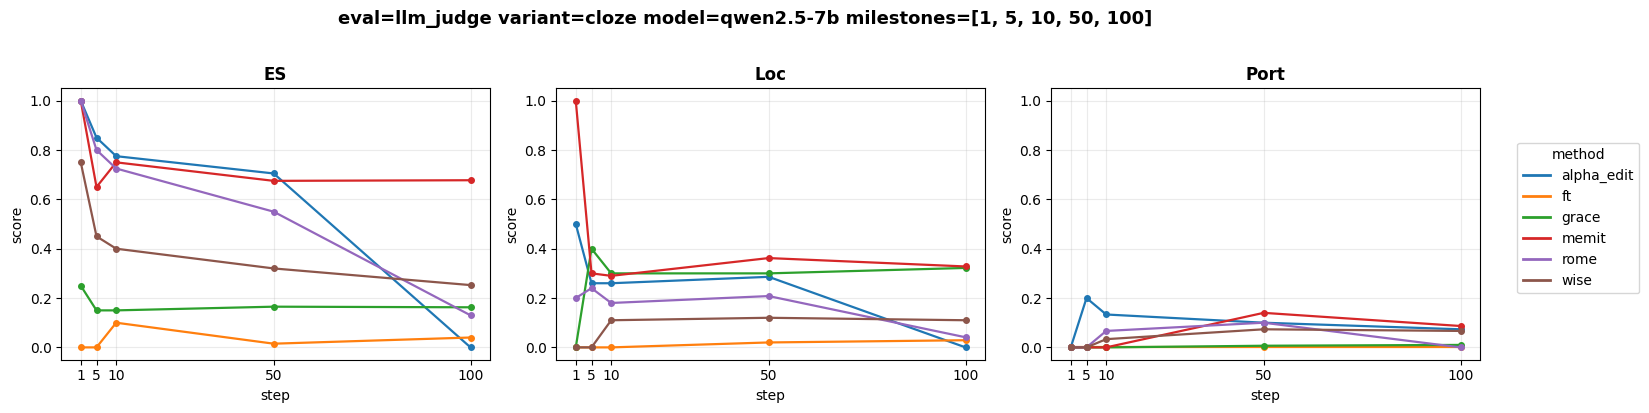
\includegraphics[width=0.9\textwidth]{figures/c4/cloze.png}
    \caption{Milestone curves for the cloze variant.}
    \label{fig:results_cloze_placeholder}
\end{figure}

\begin{figure}[H]
    \centering
    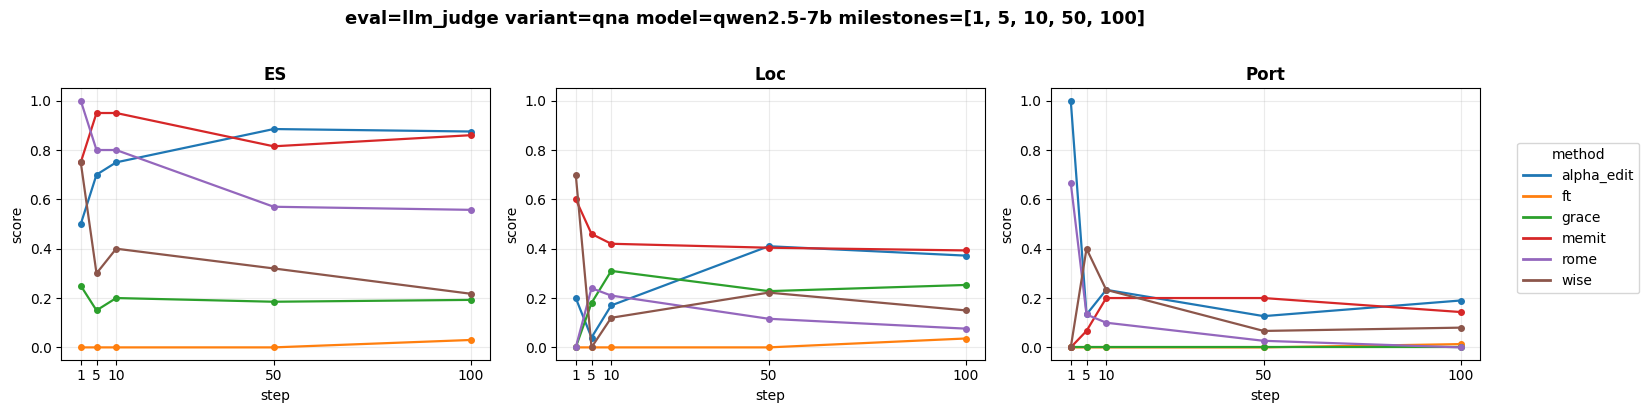
\includegraphics[width=0.9\textwidth]{figures/c4/qna.png}
    \caption{Milestone curves for the QnA variant.}
    \label{fig:results_qna_placeholder}
\end{figure}

\subsection{Interpretation of the Baselines}

The baseline comparison reveals a structural separation between the strongest editors and the most deployment-friendly ones. FT serves mainly as a collapse reference. Its poor performance from the first milestone shows that direct sequential fine-tuning on shared parameters is insufficient in the present setting. ROME is substantially more targeted and performs well at small milestones, but its repeated rank-one rewrites degrade under longer edit streams, which indicates that precise single-edit behavior does not automatically translate into stable lifelong accumulation.

MEMIT and AlphaEdit form the strongest regime in the study. Both achieve high success under paraphrased evaluation at early and medium milestones. MEMIT is the most stable method across the full 100-edit sequence, while AlphaEdit is stronger early on but collapses completely at the final milestone in the present configuration. This behavior is consistent with a broader interpretation of the two methods: MEMIT provides high-capacity multi-layer rewriting, whereas AlphaEdit adds stronger protection that can help at moderate scale but also become restrictive under longer accumulation.

GRACE and WISE remain closer to the spirit of online editing because they do not rely on repeatedly rewriting the same shared backbone weights in the same way as direct parameter-modification methods. Nevertheless, in the present experiments that structural advantage does not translate into stronger direct editing behavior. Their results remain below the strongest rewriting methods on both success and portability.

\subsection{Implications and Future Direction}

The main implication of the results is not that one existing method solves lifelong editing. Rather, the results expose a persistent trade-off between stability and editing cost. The methods that produce the strongest and most durable factual rewrites are also the methods that are more expensive, more assumption-heavy, and less convenient to apply continuously in a live environment.

The study also supports a broader hypothesis about update regimes. When several edits can be handled together, the resulting behavior is often more stable than repeated one-by-one rewriting. However, batch stability alone is not a sufficient answer for lifelong editing, because real update streams do not reveal all future edits in advance. New facts may arrive individually, may overwrite earlier temporary facts, and may need to influence the model before any expensive consolidation step is possible.

For that reason, the current research direction remains the hybrid complementary system introduced in Chapter 3. Under that view, a fast explicit component is responsible for recent and still-changeable edits, while stronger weight-rewriting methods are reserved for periodic consolidation into a stable checkpoint. The current thesis does not complete that system, but it establishes the empirical basis for why such a division is reasonable and why a single mechanism is unlikely to satisfy all requirements of lifelong editing equally well.
